\chapter{Mesure, matrices de densité et entropie}

L’expérience des deux fentes contient le problème de la mesure sous sa forme la plus simple qui soit utile. Lorsque deux possibilités restent cohérentes, leurs amplitudes interfèrent. Lorsqu’un autre système garde une trace de la possibilité réalisée, l’objet et l’enregistreur s’intriquent, et l’interférence change. Nous allons décrire ce mécanisme avec précision avant d’introduire la trace, la matrice de densité et l’entropie---les outils nécessaires pour quantifier l’intrication.

\section{Reconstruction de l’expérience des deux fentes}

Considérons un modèle discret avec une source au site \(0\), deux ouvertures \(A\) et \(B\), et un écran dont les sites d’arrivée possibles sont représentés par des états orthonormés \(\{|m\rangle\}\). La particule peut être un électron, un photon ou tout autre objet quantique. Nous l’appellerons électron et négligerons son spin propre, de sorte que seule sa position soit considérée ici. Le reste de la barrière est fermé : tout électron qui atteint un site autre que \(A\) ou \(B\) est réfléchi.

Le principe fondamental est la linéarité. Si deux états évoluent selon
\begin{equation}
|A\rangle\longrightarrow |A'\rangle,
\qquad
|B\rangle\longrightarrow |B'\rangle,
\end{equation}
alors toute superposition évolue avec les mêmes coefficients :
\begin{equation}
\alpha|A\rangle+\beta|B\rangle
\longrightarrow
\alpha|A'\rangle+\beta|B'\rangle.
\end{equation}

Dans une configuration symétrique, la source alimente les deux ouvertures avec la même amplitude. Comme au tableau, omettons le facteur de normalisation commun :
\begin{equation}
|0\rangle\longrightarrow |A\rangle+|B\rangle.
\end{equation}
L’état normalisé serait \((|A\rangle+|B\rangle)/\sqrt{2}\) ; le facteur omis ne joue aucun rôle dans l’argument relatif aux interférences.

Étudions maintenant chaque trajet séparément. La propagation des ouvertures jusqu’à l’écran s’écrit
\begin{align}
|A\rangle &\longrightarrow \sum_m \psi_m|m\rangle, \\
|B\rangle &\longrightarrow \sum_m \phi_m|m\rangle.
\end{align}
Le nombre complexe \(\psi_m\) est l’amplitude d’arrivée au site \(m\) de l’écran pour un départ de \(A\), et \(\phi_m\) est l’amplitude correspondante pour un départ de \(B\).

\begin{figure}[htbp]
\centering
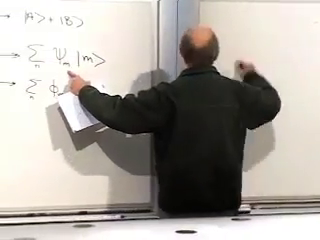
\includegraphics[width=0.68\textwidth]{lecture_07_figure_02.png}
\caption{Développements séparés des trajets \(A\) et \(B\) dans la base de l’écran.}
\lectureframe{00:05:39}
\end{figure}

Si \(B\) est fermée, la probabilité au site \(m\) vaut
\begin{equation}
P_A(m)=|\psi_m|^2.
\end{equation}
Si \(A\) est fermée,
\begin{equation}
P_B(m)=|\phi_m|^2.
\end{equation}
La probabilité classique suggérerait d’additionner ces deux résultats lorsque les deux ouvertures sont accessibles. En mécanique quantique, on additionne d’abord les amplitudes :
\begin{equation}
|A\rangle+|B\rangle
\longrightarrow
\sum_m(\psi_m+\phi_m)|m\rangle.
\end{equation}
En un site donné de l’écran,
\begin{align}
P(m)
&=|\psi_m+\phi_m|^2 \\
&=|\psi_m|^2+|\phi_m|^2
  +\psi_m^*\phi_m+\phi_m^*\psi_m.
\end{align}

\begin{figure}[htbp]
\centering
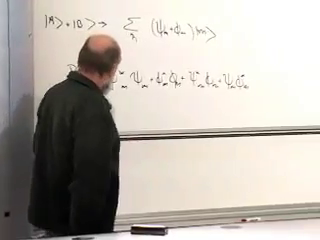
\includegraphics[width=0.70\textwidth]{lecture_07_figure_03.png}
\caption{La probabilité à l’écran comporte quatre termes. Les deux derniers sont les termes d’interférence.}
\lectureframe{00:09:21}
\end{figure}

En un point de symétrie, \(\psi_m=\phi_m\), et les deux possibilités se renforcent mutuellement. En un point où leurs phases diffèrent de \(\pi\), \(\psi_m=-\phi_m\), la probabilité s’annule. Chacun des trajets, pris séparément, peut mener à ce point ; pourtant, ouvrir les deux trajets peut empêcher l’électron d’y arriver. La question s’impose alors : qu’est-ce qui change lorsqu’un dispositif enregistre l’ouverture empruntée ?

\section{Un détecteur s’intrique avec le système}

Introduisons un système auxiliaire à deux états, \(|u\rangle\) et \(|d\rangle\). Dans ce modèle, il ne s’agit pas du spin de l’électron, mais d’un appareil externe minimal. Au départ, le détecteur n’est pas déclenché :
\begin{equation}
|0,d\rangle.
\end{equation}
Organisons l’interaction de sorte que le passage par \(A\) retourne l’état du détecteur, tandis que le passage par \(B\) le laisse inchangé :
\begin{equation}
|0,d\rangle
\longrightarrow
|A,u\rangle+|B,d\rangle.
\end{equation}
Après que l’électron a quitté les ouvertures, il n’interagit plus avec le spin auxiliaire. Les deux branches se propagent donc ainsi :
\begin{align}
|A,u\rangle &\longrightarrow \sum_m\psi_m|m,u\rangle, \\
|B,d\rangle &\longrightarrow \sum_m\phi_m|m,d\rangle,
\end{align}
et l’état final est
\begin{equation}
|\Psi\rangle
=\sum_m\left(\psi_m|m,u\rangle+\phi_m|m,d\rangle\right).
\end{equation}
Le trajet et l’enregistrement du détecteur sont désormais intriqués. La lecture du détecteur révélerait l’ouverture empruntée.

\begin{classroomqa}
\lecturetimestamp{00:13:24}
\audiencequestion{Le paquet d’ondes s’est-il déjà effondré lorsque le spin bascule ?}
\lecturerresponse{Pour l’électron seul, on peut parler d’effondrement : les possibilités de trajet n’interfèrent plus. Cependant, pour le système complet formé de l’électron--et du détecteur, aucune branche n’a été éliminée. L’état reste \(|A,u\rangle+|B,d\rangle\). En incluant l’appareil, on remplace l’affirmation \emph{l’électron s’est effondré} par la formulation précise : une intrication entre le système--et l’appareil s’est établie.}
\end{classroomqa}

Le spin auxiliaire n’est qu’un pointeur commode. Un dispositif déclenché ou non, un photon émis ou absent, ou toute autre paire d’enregistrements distinguables peut jouer le même rôle.

\begin{classroomqa}
\lecturetimestamp{00:15:17}
\audiencequestion{Le simple passage à travers la plaque métallique laisse-t-il toujours une trace du trajet ?}
\lecturerresponse{Pas nécessairement. Ce qui compte, c’est que l’interaction laisse la plaque dans des états finaux distinguables. Si la plaque possède une énergie de seuil pour ses excitations et que l’électron n’a pas assez d’énergie pour en produire une, aucune marque interne durable n’est nécessairement laissée. Une simple interaction ne suffit pas : les deux possibilités doivent se corréler avec des enregistrements distinguables.}
\end{classroomqa}

\begin{classroomqa}
\lecturetimestamp{00:16:29}
\audiencequestion{Le recul de la plaque pourrait-il révéler si l’électron est passé par l’ouverture supérieure ou inférieure ?}
\lecturerresponse{Seulement si les impulsions opposées produisent des états de la plaque suffisamment distinguables. Une plaque bien localisée possède déjà une fonction d’onde en impulsion étalée. De petits déplacements vers le haut et vers le bas peuvent se recouvrir presque complètement : les états de recul ne sont alors pas orthogonaux et ne fournissent pas d’enregistrement univoque du trajet. C’est ici que le principe d’incertitude protège les interférences.}
\end{classroomqa}

Un enregistrement partiel est possible. Si le détecteur ne reçoit qu’une faible impulsion, les deux états finaux de l’enregistrement ne sont pas nécessairement orthogonaux. L’interférence est alors réduite, mais pas éliminée. Pour le calcul formel, commençons par le cas limite d’une mesure complète :
\begin{equation}
\langle u|d\rangle=0.
\end{equation}

\section{Calcul à l’aide du projecteur}

Calculons maintenant la probabilité que l’électron arrive en un site donné \(m\) de l’écran, sans chercher à connaître le résultat de la mesure du détecteur. Dans l’espace de Hilbert combiné, la propriété \emph{électron en \(m\)} correspond à un sous-espace de dimension deux, engendré par
\begin{equation}
|m,u\rangle,\qquad |m,d\rangle.
\end{equation}
Le projecteur correspondant est
\begin{equation}
\Pi_m
=|m,u\rangle\langle m,u|
 +|m,d\rangle\langle m,d|.
\end{equation}

\begin{figure}[htbp]
\centering
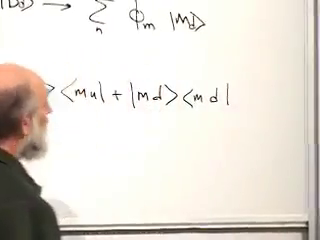
\includegraphics[width=0.66\textwidth]{lecture_07_figure_04.png}
\caption{Le projecteur sur une position donnée de l’écran, sommé sur les deux enregistrements orthogonaux du détecteur.}
\lectureframe{00:22:04}
\end{figure}

Le postulat des probabilités donne
\begin{equation}
P(m)=\langle\Psi|\Pi_m|\Psi\rangle.
\end{equation}
En développant les sommes,
\begin{align}
P(m)
&=
\sum_{n,n'}
\left(\psi_n^*\langle n,u|+\phi_n^*\langle n,d|\right)
\notag\\
&\quad\times\Pi_m
\notag\\
&\quad\times
\left(\psi_{n'}|n',u\rangle+\phi_{n'}|n',d\rangle\right).
\end{align}
Les produits scalaires de position imposent la condition \(n=m=n'\). Les produits scalaires entre états du détecteur déterminent alors quels termes subsistent :
\begin{align}
\langle u|u\rangle&=1,
&
\langle d|d\rangle&=1,
&
\langle u|d\rangle&=\langle d|u\rangle=0.
\end{align}
On obtient donc
\begin{equation}
P(m)=|\psi_m|^2+|\phi_m|^2.
\end{equation}

Les termes croisés n’ont pas été éliminés par décret. Ils s’annulent parce que les deux amplitudes de trajet multiplient désormais des vecteurs orthogonaux dans l’espace d’états élargi. Pour qu’il y ait interférence, les possibilités doivent coïncider non seulement au point d’arrivée sur l’écran, mais aussi dans chaque degré de liberté qui porte une trace.

\section{Qu’est-ce qui constitue une mesure ?}

Le modèle simple du spin fournit une règle générale : il y a mesure lorsqu’une interaction établit une corrélation entre les possibilités du système et des états distinguables d’un appareil. Les variantes suivantes permettent de mettre cette règle à l’épreuve.

\begin{classroomqa}
\lecturetimestamp{00:26:53}
\audiencequestion{Que se passe-t-il si le spin est placé symétriquement et bascule au passage par l’une ou l’autre ouverture ?}
\lecturerresponse{Les deux branches portent alors le même enregistrement, \(|A,u\rangle+|B,u\rangle=(|A\rangle+|B\rangle)\otimes|u\rangle\). L’état du détecteur se factorise et ne révèle aucune information sur le trajet ; la figure d’interférence est donc conservée.}
\end{classroomqa}

\begin{figure}[htbp]
\centering
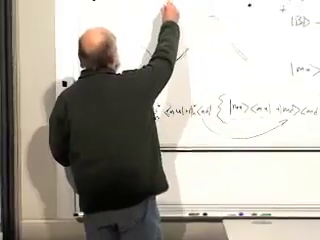
\includegraphics[width=0.68\textwidth]{lecture_07_figure_05.png}
\caption{Variante au tableau : un détecteur placé symétriquement réagit de la même façon aux deux trajets.}
\lectureframe{00:27:14}
\end{figure}

\begin{figure}[htbp]
\centering
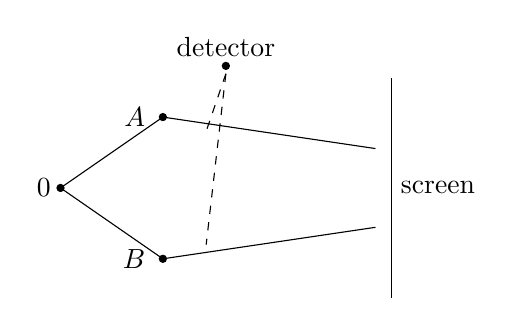
\begin{tikzpicture}[scale=1.0]
\fill (-2,0) circle (1.5pt);
\node[left] at (-2,0) {$0$};
\fill (-0.7,0.9) circle (1.5pt);
\node[left] at (-0.8,0.9) {$A$};
\fill (-0.7,-0.9) circle (1.5pt);
\node[left] at (-0.8,-0.9) {$B$};
\draw (-2,0) -- (-0.7,0.9);
\draw (-2,0) -- (-0.7,-0.9);
\draw (-0.7,0.9) -- (2.0,0.5);
\draw (-0.7,-0.9) -- (2.0,-0.5);
\draw (2.2,-1.4) -- (2.2,1.4);
\node[right] at (2.2,0) {screen};
\fill (0.1,1.55) circle (1.5pt);
\node[above] at (0.1,1.55) {detector};
\draw[dashed] (0.1,1.45) -- (-0.15,0.72);
\draw[dashed] (0.1,1.45) -- (-0.15,-0.72);
\end{tikzpicture}
\caption{Reconstitution nette du placement symétrique du détecteur : les deux trajets produisent le même état du détecteur.}
\end{figure}

\begin{classroomqa}
\lecturetimestamp{00:27:55}
\audiencequestion{Faut-il que quelqu’un lise effectivement le spin auxiliaire pour que les interférences disparaissent ?}
\lecturerresponse{Non. L’électron a déjà corrélé son trajet avec le spin. On peut réinitialiser le détecteur, répéter l’expérience électron par électron et examiner uniquement la répartition des impacts sur l’écran. Les franges ont disparu même si personne ne lit le spin ; c’est l’enregistrement physique qui compte, et non le fait qu’un humain en ait connaissance.}
\end{classroomqa}

\begin{classroomqa}
\lecturetimestamp{00:29:36}
\audiencequestion{Une plaque suffisamment légère, mise en recul, détruirait-elle les interférences ?}
\lecturerresponse{Oui, si le recul place la plaque dans des états d’impulsion orthogonaux selon le trajet. Si les paquets d’ondes déplacés se recouvrent encore, la destruction n’est que partielle. La masse à elle seule ne détermine pas le résultat : c’est le caractère distinguable des états finaux de la plaque qui compte.}
\end{classroomqa}

Le rayonnement constitue un autre enregistreur imparfait. Une particule chargée accélérée peut émettre un photon. Le rayonnement émis près de \(A\) n’est pas nécessairement dans le même état que celui émis près de \(B\) ; le champ électromagnétique peut donc conserver une information sur le trajet. Pour un électron faiblement dévié, la probabilité d’émission peut être faible ; le cours donne, à titre illustratif, une estimation d’environ un événement sur cent. Une accélération plus forte rend l’émission de rayonnement, et donc la perte de contraste, plus probable. Le point essentiel est qualitatif : même un photon non observé peut emporter de la cohérence.

\begin{classroomqa}
\lecturetimestamp{00:32:00}
\audiencequestion{Comment déduire la probabilité d’interférence dans une expérience réelle où le contraste est imparfait ?}
\lecturerresponse{On répète l’expérience de nombreuses fois et l’on estime la distribution sur l’écran à partir des fréquences relatives. Un échantillon de taille finie et les enregistrements laissés dans l’environnement produisent des impacts résiduels dans les régions normalement sombres. L’estimation de la distribution de probabilité s’améliore avec le nombre d’essais, tandis que les processus de décohérence réduisent le contraste physique des franges.}
\end{classroomqa}

\begin{classroomqa}
\lecturetimestamp{00:33:13}
\audiencequestion{Le simple fait qu’il soit possible de déterminer le trajet détruit-il toute interférence ?}
\lecturerresponse{Une distinguabilité complète la détruit entièrement. Une information partielle entraîne une perte partielle. Si un détecteur ne tourne que légèrement, les deux états d’enregistrement restent non orthogonaux : à la lecture du détecteur, un trajet devient plus probable que l’autre, sans être certain. Les franges sont donc brouillées plutôt qu’effacées.}
\end{classroomqa}

Notons \(|E_A\rangle\) et \(|E_B\rangle\) des états d’enregistrement arbitraires. L’état combiné à l’écran peut s’écrire
\begin{equation}
|\Psi\rangle
=\sum_m\left(
\psi_m|m\rangle|E_A\rangle
+\phi_m|m\rangle|E_B\rangle
\right).
\end{equation}
Si l’on ne tient pas compte du système qui conserve l’enregistrement, on obtient
\begin{align}
P(m)
&=|\psi_m|^2+|\phi_m|^2 \\
&\quad
+\psi_m^*\phi_m\langle E_A|E_B\rangle
+\phi_m^*\psi_m\langle E_B|E_A\rangle.
\end{align}
Le recouvrement \(\langle E_A|E_B\rangle\) est donc le facteur de cohérence. Des enregistrements identiques préservent toute l’interférence ; des enregistrements orthogonaux la suppriment ; un recouvrement intermédiaire donne une visibilité intermédiaire.

\begin{classroomqa}
\lecturetimestamp{00:34:12}
\audiencequestion{Si des photons ne sont émis qu’occasionnellement, que se passe-t-il si l’on ne retient que les événements avec émission d’un photon ?}
\lecturerresponse{L’interférence est généralement plus faible dans ce sous-ensemble sélectionné, car un photon porte une information sur le trajet. La perte n’est pas nécessairement complète : les paquets d’ondes des photons émis aux deux ouvertures peuvent eux-mêmes se recouvrir. Les enregistrements radiatifs peuvent donc ne pas être parfaitement orthogonaux.}
\end{classroomqa}

Le bombardement par l’environnement amplifie ce mécanisme. Les molécules d’air, les photons ambiants et la matière environnante enregistrent continuellement les positions macroscopiques. Une personne ou la Lune ne reste pas visiblement dans une superposition cohérente de positions : la masse ralentit la dispersion libre, et l’intrication continue avec l’environnement supprime les interférences observables entre possibilités macroscopiquement séparées.

\begin{classroomqa}
\lecturetimestamp{00:36:02}
\audiencequestion{S’agit-il déjà d’une théorie de la mesure, et pas seulement d’un nouvel usage de l’expression \emph{effondrement du paquet d’ondes} ?}
\lecturerresponse{C’est le mécanisme à l’œuvre dans un exemple volontairement traité avec précision. Dans une description limitée à l’électron, l’effondrement consiste à écarter les termes hors diagonale \(\psi^*\phi\). Dans la description du système composite, aucune suppression ad hoc n’est nécessaire : l’intrication avec des états orthogonaux de l’appareil rend ces termes inaccessibles aux mesures effectuées sur le seul électron. Il faut ramener les exemples plus complexes à cette structure.}
\end{classroomqa}

\begin{classroomqa}
\lecturetimestamp{00:38:04}
\audiencequestion{Un champ gravitationnel qui courbe le trajet modifierait-il naturellement l’argument sur le rayonnement ou la règle des interférences ?}
\lecturerresponse{Le rayonnement dans le détail peut changer, et la mécanique quantique n’attribue pas de trajectoire unique et bien définie avant une mesure de trajet. La conclusion générale reste la même : seule une variable qui conserve une information distinguable sur le trajet supprime les interférences. Il faut préciser l’appareil concret pour qu’une réponse plus détaillée ait un sens.}
\end{classroomqa}

\begin{classroomqa}
\lecturetimestamp{00:39:44}
\audiencequestion{Cette interférence diffère-t-elle de celle des ondes électromagnétiques classiques ?}
\lecturerresponse{Pour un grand nombre de photons, la figure observée concorde avec l’interférence ordinaire des ondes électromagnétiques. L’expérience à particule unique met en évidence l’affirmation quantique plus profonde : photons et électrons arrivent sous forme d’événements individuels, tandis que leurs amplitudes quantiques interfèrent. Pour les électrons, l’onde pertinente est la fonction d’onde de l’électron, et non une onde électromagnétique.}
\end{classroomqa}

\begin{classroomqa}
\lecturetimestamp{00:40:45}
\audiencequestion{Que deviennent les parties de l’onde initiale dirigées entre \(A\) et \(B\) ?}
\lecturerresponse{Dans ce modèle délibérément discret, le reste de la barrière est fermé. Ces parties sont réfléchies et ne contribuent pas à l’amplitude transmise jusqu’à l’écran. Le modèle isole les deux possibilités transmises sans prétendre qu’un faisceau réel ne possède que deux composantes d’impulsion.}
\end{classroomqa}

\section{Le chat, l’écran et la frontière mobile}

Les mêmes mathématiques s’appliquent au chat de Schr\"odinger. Notons \(|U\rangle\) et \(|F\rangle\) les états du pistolet, respectivement non déclenché et déclenché, et \(|L\rangle\) et \(|D\rangle\) les états du chat, vivant et mort. En partant d’un chat vivant et d’un pistolet non déclenché, l’interaction peut produire
\begin{equation}
|\Psi_{\mathrm{cat}}\rangle
=\alpha|L,U\rangle+\beta|D,F\rangle.
\end{equation}
Le chat seul n’est pas dans l’état cohérent \(\alpha|L\rangle+\beta|D\rangle\). Il est intriqué avec un pistolet qui a enregistré la possibilité réalisée. Examiner le pistolet peut révéler la branche du chat, et les enregistrements orthogonaux du pistolet suppriment l’interférence ordinaire entre vivant--et mort dans le sous-système du chat.

\begin{classroomqa}
\lecturetimestamp{00:41:18}
\audiencequestion{Le chat lui-même est-il dans une superposition de vivant et de mort ?}
\lecturerresponse{Pas dans le sens simple d’un système isolé. Le système composite formé du chat--et du pistolet est dans une superposition de possibilités corrélées : vivant avec pistolet non déclenché et mort avec pistolet déclenché. Le sous-système du chat est intriqué avec un pistolet qui porte un enregistrement, exactement comme le trajet de l’électron est intriqué avec le spin auxiliaire.}
\end{classroomqa}

L’écran final doit lui aussi être traité comme un appareil. Un électron qui arrive en \(m\) peut noircir un grain photographique, faire émettre un photon par un scintillateur ou retourner l’état d’un détecteur parmi une rangée de dispositifs locaux à deux états. La marque se corrèle avec la position d’arrivée.

\begin{classroomqa}
\lecturetimestamp{00:43:38}
\audiencequestion{Pourquoi peut-on parler de probabilités sur l’écran final au lieu de ne considérer que des vecteurs d’état indéfiniment ?}
\lecturerresponse{Le postulat des probabilités associe \(\langle\Pi_m\rangle\) à la propriété \emph{arrivée en \(m\)}. Pour compléter l’expérience physique, l’écran laisse ensuite une trace de la position. Le projecteur donne la probabilité ; le noircissement, la scintillation ou le basculement d’un détecteur local réalise la mesure dont on recueille les statistiques.}
\end{classroomqa}

\begin{classroomqa}
\lecturetimestamp{00:45:00}
\audiencequestion{Pourquoi parler d’une mesure sur l’écran, mais pas d’une probabilité de passage par \(A\) ou \(B\) ?}
\lecturerresponse{On ne peut attribuer et vérifier des probabilités de trajet qu’en installant un enregistreur de trajet. Sans un tel enregistrement, les possibilités restent cohérentes et doivent être additionnées sous forme d’amplitudes. On suppose que l’écran est muni d’un appareil sensible à la position. La différence ne tient pas à un instant privilégié, mais à la mise en place ou non d’une interaction de mesure correspondante.}
\end{classroomqa}

On peut déplacer la frontière entre le système et l’appareil. Incluons un observateur ayant pour états d’enregistrement \(|O_u\rangle\) et \(|O_d\rangle\) ; on a alors
\begin{equation}
|A,u\rangle+|B,d\rangle
\longrightarrow
|A,u,O_u\rangle+|B,d,O_d\rangle.
\end{equation}
Un autre observateur peut à son tour se corréler avec le premier. La fumée dans la boîte du chat, le pistolet, le chat, Schr\"odinger et Wigner peuvent tous être inclus dans une chaîne d’intrication plus longue. Quel que soit l’endroit où l’on place la frontière, les corrélations doivent rester cohérentes : si Wigner demande ensuite Schr\"odinger ce qu’il a vu, leurs enregistrements concordent.

\begin{classroomqa}
\lecturetimestamp{00:47:24}
\audiencequestion{Où faut-il exactement arrêter le système et faire commencer l’observateur qui mesure ?}
\lecturerresponse{La mécanique quantique ne fixe aucune frontière unique et commode. On peut faire s’effondrer la description de l’électron seul, inclure le détecteur et faire s’effondrer une description plus large, ou inclure un observateur et élargir encore l’état intriqué. L’exigence physique est la cohérence de toutes les probabilités et de tous les enregistrements accessibles, et non l’existence d’une frontière comptable unique.}
\end{classroomqa}

\begin{classroomqa}
\lecturetimestamp{00:49:47}
\audiencequestion{Le principe d’incertitude intervient-il parce que la mesure du trajet perturbe l’événement ?}
\lecturerresponse{Oui. L’exemple du recul établit clairement le lien : la localisation de la plaque entraîne une incertitude sur son impulsion, qui peut empêcher de distinguer de petites impulsions dépendant du trajet. Plus généralement, une mesure quantique n’est complète que lorsque l’intrication entre système--et appareil a modifié l’état, et cette modification peut changer le résultat d’une expérience d’interférence ultérieure.}
\end{classroomqa}

Cela marque un contraste net avec l’idéal classique. Classiquement, on imagine pouvoir effectuer une mesure arbitrairement douce et recueillir de l’information avec une perturbation négligeable. Ici, obtenir une information sur le trajet exige d’établir une corrélation avec un appareil. Cela modifie réellement l’état conjoint et change le résultat d’une expérience d’interférence ultérieure.

\begin{classroomqa}
\lecturetimestamp{00:52:06}
\audiencequestion{Que se passe-t-il si la distance entre \(A\) et \(B\) devient très grande ?}
\lecturerresponse{Il n’existe pas de nouvelle règle universelle. Dans cette géométrie avec source et barrière, les amplitudes d’arrivée aux ouvertures très éloignées peuvent simplement devenir faibles, de sorte que la plupart des particules frappent la région obstruée. Hormis ces changements qui dépendent de l’appareil et affectent \(\psi_m\) et \(\phi_m\), la distance à elle seule ne détermine pas si la cohérence subsiste.}
\end{classroomqa}

\begin{classroomqa}
\lecturetimestamp{00:53:04}
\audiencequestion{La linéarité de l’évolution quantique est-elle fondamentalement exacte, et pourquoi la nature l’utilise-t-elle ?}
\lecturerresponse{La linéarité est un fondement empirique de la mécanique quantique. De petites modifications non linéaires sont notoirement difficiles à rendre cohérentes sur le plan logique et tendent à dégrader la structure. La raison profonde pour laquelle les propositions physiques suivent la logique des sous-espaces plutôt que celle des ensembles classiques n’est pas donnée ici ; le cours la considère comme un fait de la nature.}
\end{classroomqa}

\begin{classroomqa}
\lecturetimestamp{00:54:53}
\audiencequestion{Une observation ultérieure pourrait-elle révéler le trajet antérieur et ainsi modifier le fait qu’il y ait eu interférence ?}
\lecturerresponse{Si une observation ultérieure peut révéler le trajet, une variable physique a nécessairement conservé une trace dépendant du trajet. Cette trace affecte déjà la cohérence ; personne n’a besoin de la lire. Il faut néanmoins respecter la causalité, et une affirmation abstraite sur le choix retardé ne peut être tranchée sans préciser l’ensemble de la configuration spatiotemporelle et l’appareil.}
\end{classroomqa}

\begin{classroomqa}
\lecturetimestamp{00:56:47}
\audiencequestion{Que se passe-t-il si l’on place une chambre à bulles juste après les ouvertures ?}
\lecturerresponse{Une trajectoire qui distingue les deux trajets à la sortie constitue une marque sans équivoque et détruit donc leur interférence. Une fine couche qui enregistre le trajet suffit. Si un dispositif en aval ne conserve pas assez d’information pour déduire l’ouverture empruntée auparavant, il ne joue pas automatiquement le rôle de détecteur du trajet.}
\end{classroomqa}

\begin{classroomqa}
\lecturetimestamp{00:59:29}
\audiencequestion{Si le monde est déjà fortement intriqué, comment une expérience d’interférence peut-elle commencer avec des systèmes non intriqués ?}
\lecturerresponse{La préparation doit isoler, réinitialiser ou sélectionner les degrés de liberté pertinents avec suffisamment de soin pour que les possibilités commencent avec le même enregistrement environnemental. On ne peut pas simplement ignorer une trace antérieure dans une chambre à bulles si elle reste corrélée au trajet. L’interférence exige au départ une relation de type produit entre le système contrôlé et l’enregistreur pertinent.}
\end{classroomqa}

\begin{classroomqa}
\lecturetimestamp{01:01:04}
\audiencequestion{Comment obtient-on une désintrication pratique après une mesure ?}
\lecturerresponse{Conditionnons sur un résultat observé déterminé. Si le spin est mesuré vers le haut, l’observateur conserve la branche \(|A,u\rangle\) et écarte l’autre possibilité de sa description de travail. Cet état produit conditionnel peut servir de nouveau point de départ. L’état complet qui inclut l’observateur peut rester intriqué, mais, relativement au résultat enregistré, la préparation sélectionnée est déterminée.}
\end{classroomqa}

Cette hiérarchie imbriquée ne résout pas toutes les questions d’interprétation, mais elle rend visible la cohérence opérationnelle. On peut inclure le système, le détecteur, l’observateur et l’observateur de l’observateur. Quel que soit l’endroit où l’on arrête la description, des enregistrements correctement corrélés ne se contredisent pas par la suite.

\section{De l’intrication à l’entropie}

La discussion sur la mesure est allée plus loin que prévu, mais elle a fait apparaître la question suivante : comment mesurer le degré d’intrication ? Deux spins dans l’état produit
\begin{equation}
|u\rangle\otimes|u\rangle
\end{equation}
ne sont pas intriqués. Chaque sous-système possède son propre état déterminé, et l’observation de l’un n’apporte aucune information nouvelle sur l’autre. Les états intriqués ne se factorisent pas ainsi. L’entropie d’intrication constitue un diagnostic quantitatif standard, mais il faut d’abord introduire la notion ordinaire d’entropie, puis sa forme quantique.

\section{L’entropie classique comme information manquante}

Commençons par un système classique qui possède un ensemble fini de \(N\) états possibles. Ici, l’entropie est une propriété du système conjuguée à ce que nous en savons. Supposons que tout ce que nous sachions soit que le système occupe l’un de \(n\) états équiprobables. Alors
\begin{equation}
S=\log n.
\end{equation}
Si \(n=1\), l’état est connu et \(S=0\). Si \(n=N\), on ne sait rien au-delà de l’espace des états lui-même et l’entropie est maximale : \(S_{\max}=\log N\).

Le logarithme rend additive la comptabilisation des choix indépendants entre oui--et non. Pour \(M\) spins classiques, il existe \(2^M\) configurations, donc
\begin{equation}
\log(2^M)=M\log 2.
\end{equation}
À un choix près de la base du logarithme, l’entropie mesure ainsi la quantité d’information binaire manquante dans la description.

Pour une distribution de probabilité générale \(p_i\), la définition appropriée est
\begin{equation}
S=-\sum_i p_i\log p_i.
\end{equation}

\begin{classroomqa}
\lecturetimestamp{01:14:17}
\audiencequestion{Pourquoi y a-t-il un signe moins dans la formule de l’entropie ?}
\lecturerresponse{Toute probabilité non nulle vérifie \(0<p_i\leq 1\), donc \(\log p_i\leq 0\). Le signe moins rend l’entropie non négative. Pour \(p_i=0\), la contribution est définie par la limite \(p_i\log p_i\to0\).}
\end{classroomqa}

Pour la distribution équiprobable
\begin{equation}
p_i=
\begin{cases}
1/n, & i\in\mathcal N,\\
0, & i\notin\mathcal N,
\end{cases}
\qquad |\mathcal N|=n,
\end{equation}
la formule générale devient
\begin{align}
S
&=-n\left(\frac1n\right)\log\left(\frac1n\right)\\
&=\log n.
\end{align}
Elle redonne donc la définition élémentaire par dénombrement. Une distribution qui se concentre avec certitude sur un seul état a pour entropie \(S=0\).

\begin{figure}[htbp]
\centering
\includegraphics[width=0.66\textwidth]{lecture_07_figure_07.png}
\caption{Le tableau récapitule \(S=\log n\), la formule de Shannon et le cas équiprobable.}
\lectureframe{01:16:08}
\end{figure}

\begin{classroomqa}
\lecturetimestamp{01:17:35}
\audiencequestion{Quelle est l’entropie maximale d’un système à \(N\) états, et que sait-on dans ce cas ?}
\lecturerresponse{Le maximum vaut \(\log N\) et est atteint pour la distribution uniforme \(p_i=1/N\). On sait toujours de quel système il s’agit et l’on connaît donc son espace d’états ; ce qui reste inconnu, c’est lequel de ces \(N\) états il occupe.}
\end{classroomqa}

La différence
\begin{equation}
I=S_{\max}-S
\end{equation}
représente l’information disponible au sens de ce dénombrement. Entropie et information sont les deux faces d’une même comptabilité : l’entropie quantifie l’information qui permettrait de distinguer l’état, mais dont nous ne disposons pas.

\section{La trace : le remplacement quantique d’une somme}

Pour un opérateur \(M\) et une base orthonormée complète quelconque \(\{|i\rangle\}\), définissons
\begin{equation}
\operatorname{Tr}M
=\sum_i\langle i|M|i\rangle.
\end{equation}

\begin{figure}[htbp]
\centering
\includegraphics[width=0.68\textwidth]{lecture_07_figure_08.png}
\caption{La trace écrite comme somme des éléments diagonaux de la matrice.}
\lectureframe{01:21:20}
\end{figure}

Bien que la définition soit formulée à l’aide d’une base, le résultat est indépendant de celle-ci. Pour un opérateur hermitien, on peut choisir une base propre, dans laquelle
\begin{equation}
\operatorname{Tr}M=\sum_i\lambda_i.
\end{equation}
Les valeurs propres, et donc leur somme, ne dépendent pas des coordonnées utilisées pour représenter l’opérateur.

\begin{classroomqa}
\lecturetimestamp{01:23:04}
\audiencequestion{Le fait de mettre une matrice sous forme diagonale implique-t-il qu’elle possède un inverse ?}
\lecturerresponse{Non. La forme diagonale fait apparaître les valeurs propres ; l’inversibilité est une condition distincte. Une matrice diagonale est inversible si et seulement si aucune de ses valeurs propres diagonales n’est nulle. Les matrices hermitiennes sont diagonalisables même lorsque certaines valeurs propres s’annulent.}
\end{classroomqa}

Après la pause, revenons brièvement aux probabilités classiques. Une observable classique est une fonction \(f_i\) de la configuration, et sa moyenne vaut
\begin{equation}
\langle f\rangle_{\mathrm{cl}}=\sum_i p_i f_i.
\end{equation}
Dans les formules quantiques, la trace remplacera la somme sur les possibilités, un opérateur remplacera la fonction classique, et une matrice densité remplacera la distribution de probabilité.

\section{Mélanges statistiques et matrice densité}

Supposons qu’une personne prépare un système dans l’un des états d’une base orthonormée, sans nous dire lequel a été choisi. Elle ne fournit que les probabilités de préparation--- : par exemple, un spin est préparé dans l’état « vers le haut » avec une probabilité \(3/4\) et dans l’état « vers le bas » avec une probabilité \(1/4\). Il ne s’agit pas de la superposition cohérente
\begin{equation}
\sqrt{\frac34}|u\rangle+\sqrt{\frac14}|d\rangle,
\end{equation}
car aucune phase relative n’a été préparée. Il s’agit d’un mélange statistique d’états bien définis. Les probabilités quantiques subsistent même lorsque l’état pur est connu ; ici s’y ajoute une incertitude sur l’état pur qui a été préparé.

\begin{figure}[htbp]
\centering
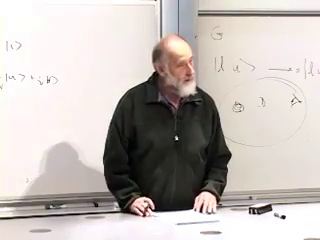
\includegraphics[width=0.66\textwidth]{lecture_07_figure_06.png}
\caption{Transition conceptuelle d’un ket spécifié à une description d’ensemble.}
\lectureframe{01:29:43}
\end{figure}

Si l’état \(|i\rangle\) est préparé avec une probabilité \(\rho_i\), l’opérateur densité est
\begin{equation}
\rho=\sum_i\rho_i|i\rangle\langle i|.
\end{equation}
Dans la base de préparation,
\begin{equation}
\rho=
\begin{pmatrix}
\rho_1&0&0&\cdots\\
0&\rho_2&0&\cdots\\
0&0&\rho_3&\cdots\\
\vdots&\vdots&\vdots&\ddots
\end{pmatrix}.
\end{equation}

\begin{figure}[htbp]
\centering
\includegraphics[width=0.68\textwidth]{lecture_07_figure_09.png}
\caption{La matrice densité diagonale et sa condition de normalisation.}
\lectureframe{01:32:12}
\end{figure}

Ses valeurs propres sont réelles et positives ou nulles, et la normalisation des probabilités s’écrit
\begin{equation}
\operatorname{Tr}\rho=\sum_i\rho_i=1.
\end{equation}

Soit \(F\) une observable hermitienne. La valeur moyenne dans l’ensemble est
\begin{equation}
\langle F\rangle=\operatorname{Tr}(F\rho).
\end{equation}

\begin{figure}[htbp]
\centering
\includegraphics[width=0.68\textwidth]{lecture_07_figure_10.png}
\caption{La valeur moyenne par la trace \(\langle F\rangle=\operatorname{Tr}(F\rho)\).}
\lectureframe{01:35:05}
\end{figure}

Pour retrouver la moyenne pondérée ordinaire, calculons la trace dans la base où \(\rho\) est diagonale et insérons la résolution de l’identité :
\begin{align}
\operatorname{Tr}(F\rho)
&=\sum_i\langle i|F\rho|i\rangle\\
&=\sum_{i,j}\langle i|F|j\rangle
               \langle j|\rho|i\rangle\\
&=\sum_i\rho_i\langle i|F|i\rangle.
\end{align}
Ainsi, la valeur moyenne dans chaque état pur est pondérée par la probabilité que l’état correspondant ait été préparé.

La trace possède la propriété cyclique
\begin{equation}
\operatorname{Tr}(AB)=\operatorname{Tr}(BA),
\end{equation}
même si \(A\) et \(B\) ne commutent pas. On a donc \(\operatorname{Tr}(F\rho)=\operatorname{Tr}(\rho F)\).

\section{Entropie quantique et bénéfice différé}

L’entropie d’une matrice densité est
\begin{equation}
S(\rho)=-\operatorname{Tr}(\rho\log\rho).
\end{equation}
Pour un opérateur hermitien positif, les fonctions telles que \(\log\rho\) sont définies à partir de ses valeurs propres. Si
\begin{equation}
\rho=\sum_i\rho_i|i\rangle\langle i|,
\end{equation}
alors
\begin{equation}
\log\rho=\sum_{\rho_i>0}(\log\rho_i)|i\rangle\langle i|,
\end{equation}
et donc
\begin{equation}
S(\rho)=-\sum_i\rho_i\log\rho_i.
\end{equation}

\begin{figure}[htbp]
\centering
\includegraphics[width=0.68\textwidth]{lecture_07_figure_11.png}
\caption{La formule classique de l’entropie réécrite sous la forme \(S=-\operatorname{Tr}(\rho\log\rho)\).}
\lectureframe{01:41:25}
\end{figure}

Un état pur connu a pour opérateur densité
\begin{equation}
\rho_\psi=|\psi\rangle\langle\psi|,
\end{equation}
dont les valeurs propres sont \(1,0,\ldots\) ; par conséquent, \(S(\rho_\psi)=0\). Cela ne signifie pas que toute mesure effectuée sur \(|\psi\rangle\) donne un résultat certain. Cela signifie qu’il n’y a pas d’ignorance statistique supplémentaire quant à l’état préparé. À l’autre extrême,
\begin{equation}
\rho=\frac{I}{d}
\qquad\Longrightarrow\qquad
S(\rho)=\log d,
\end{equation}
où \(d=\dim\mathcal H\). L’état maximalement mélangé attribue le même poids à toutes les directions orthogonales.

Le lien avec l’intrication est maintenant proche, mais il n’a pas encore été établi. Supposons qu’un système composite \(AB\) soit dans un état conjoint et que toutes les expériences se limitent à \(A\). Il doit exister un objet qui reproduit toutes les valeurs moyennes accessibles sur \(A\) lorsque \(B\) est ignoré. Cet objet est une matrice densité pour \(A\). Si l’état conjoint se factorise, la matrice densité de \(A\) est pure et son entropie est nulle. Si \(A\) et \(B\) sont intriqués, la matrice densité de \(A\) est généralement mixte et son entropie est non nulle. La construction de cette matrice densité réduite et le calcul de son entropie sont réservés au prochain cours.
